\documentclass[titlepage]{article}

\usepackage[margin=1in]{geometry}
% some more shit for the title
\usepackage[T1]{fontenc}
\usepackage{babel}

% Tables and stopping them from displaying in a different section
\usepackage{booktabs}
\usepackage[section]{placeins}

% for inserting images into the document, setting file path, and allowing rotation of inserted images 
\usepackage{graphicx}
\graphicspath{ {./images/} }
\usepackage{rotating}
\usepackage[table]{xcolor}
% mostly just for putting text in math equations
\usepackage{amsmath}
% for aligning the text to the left
\usepackage[document]{ragged2e}

% for inserting hyperlinks in the document, use \url{url} or \href{url}{text}
\usepackage{hyperref}
\usepackage{calligra}
\usepackage[T1]{fontenc}
\usepackage{siunitx}
\usepackage{caption}
\usepackage{multirow}
\usepackage[export]{adjustbox}
\usepackage{tikz}
\usepackage{pgfplots}
\pgfplotsset{soldot/.style={color=black,only marks,mark=*},
	             holdot/.style={color=black,fill=white,only marks,mark=*},
		                  compat=1.12}
\usepackage{paracol}

\begin{document}
\title{\textbf{Lab 5: Resistors in Series and Parallel}}
\author{
    Zachary Pouska\\
    \texttt{001103193}\\
    \and
    Natalie Tran \\ 
    \texttt{000698629}\\ \\
} 

\date{PHYS 236 | Fall 2022\\
Date performed: 24/10/2022}


	\maketitle


	\section{Purpose}
    Familiarity with the behavior of resistors in both series and parallel configurations, as well as experimental verification of course material on series and parallel resistors. 

    \section{Materials} 
    \begin{itemize}
        \item Handheld Digital Multimeter (DMM)
        \item Breadboard
        \item Assorted Resistors (270$\Omega$, 330$\Omega$, and 510$\Omega$)
        \item Power Supply
        \item Wires
        \item Alligator Clips
    \end{itemize}


	\section{Theory}	
    In this lab, we make use of the \textbf{ammeter} function in our digital multimeters for the final section. The electrical current is measured in Amperes, which is one coulomb per second ($1.0 A = \frac{1.0C}{1.0 s}$).\\
    \vspace{5pt}
    Additionally, we made use of the most useful feature of a digital multimeter, being the \textbf{voltmeter}. With this mode, our multimeter is able to measure the potential difference between any two points with the units of volts ($\Delta V$), which gives us an idea of the difference in potential energy between two points in our circuit.\\ 
    \vspace{5pt}

    \textbf{Resistors} have the main property of "resistance", measured in Ohms ($\Omega$), which can be thought of as a ratio of Volts over Amperes, or how many volts will be dropped across the resistor for a certain amount of current. Each resistor generally has 4-6 colored bands printed onto them, which indicate the value of its resistance. All but the last two colored bands indicate numbers in decimal increments, the second to last indicates a multiplier, and the last band indicates the tolerance of the resistor with either a silver or gold band. \\ 
    \vspace{5pt}

    A \textbf{Breadboard} is a useful tool for prototyping small electric circuits, as it lets you consistently connect electrical components together without need for wire nuts or soldering. A breadboard is essentially a grid of termination points, with rows of these points connected together. Using this principle, one row of a standard breadboard can electrically connect 5 different components together in order to make more complex circuits.

    \begin{figure}[hbt!]
        \centering
        \caption{Labeled diagram of a breadboard}
        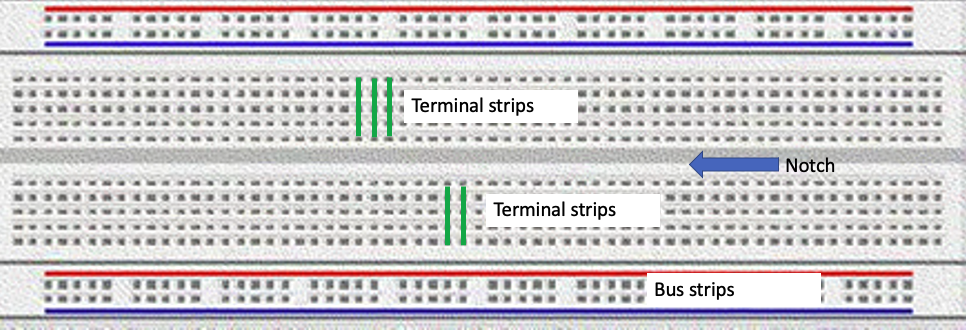
\includegraphics[scale = 0.2]{theory/breadboard}
    \end{figure} 


    \subsection*{Resistors in series}
        $$R_{eq} = R_1 +R_2 + R_3 $$
        The total Voltage across resistors in series is equal to the sum of voltage drops across each subsequent resistor. $$ V_{eq} = \varepsilon = V_1 + V_2 + V_3 = I R_1 + I R_2 + I R_3 $$

    \subsection*{Resistors in parallel} 
        $$R_{eq} = \left( \frac{1}{R_1} + \frac{1}{R_2} + \frac{1}{R_2} \right)  $$
        The voltage drop across each resistor in a parallel setup is equal to the potential difference of the battery $\varepsilon$.
        $$V_{eq} = \varepsilon = V_1 = V_2 = V_3 $$


	\section{Experiment Analysis}
    When we have resistors in parallel, the potential difference across them are the same. 
    



	\section{Procedure}
        \subsection{Measurement of the resistors using DMM}

        \begin{figure}[hbt!]
                \centering
                \caption{Six labeled resistors on a breadboard}
                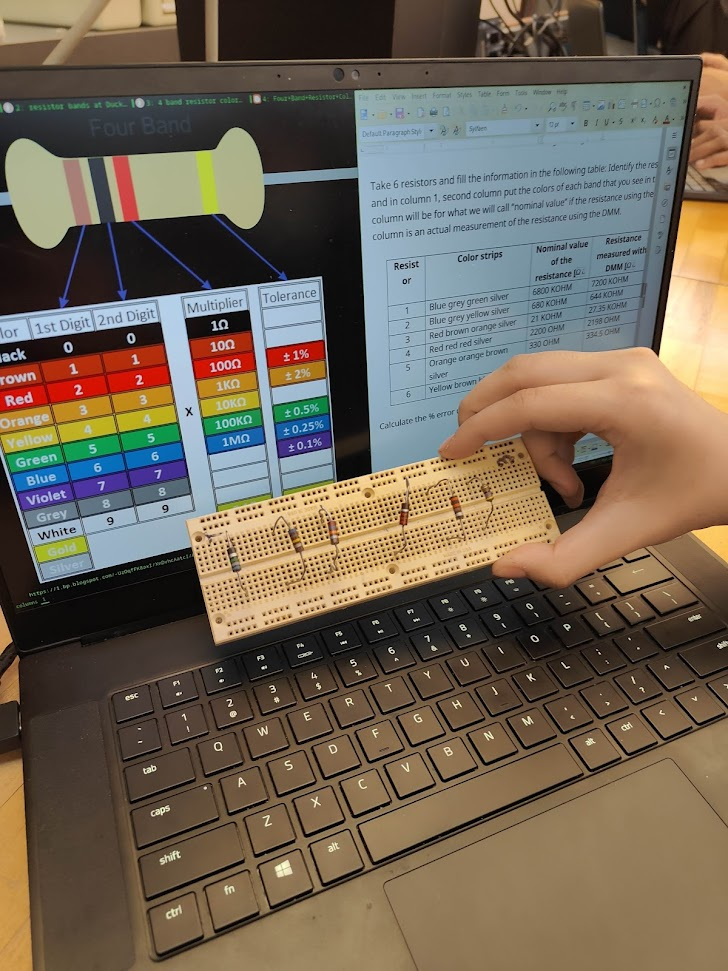
\includegraphics[scale=0.2]{procedure/unknownresistors}
            \end{figure} 


        \subsection{Series Circuit}

        \begin{figure}[hbt!]
            \centering
            \caption{Resistors in a series configuration}
    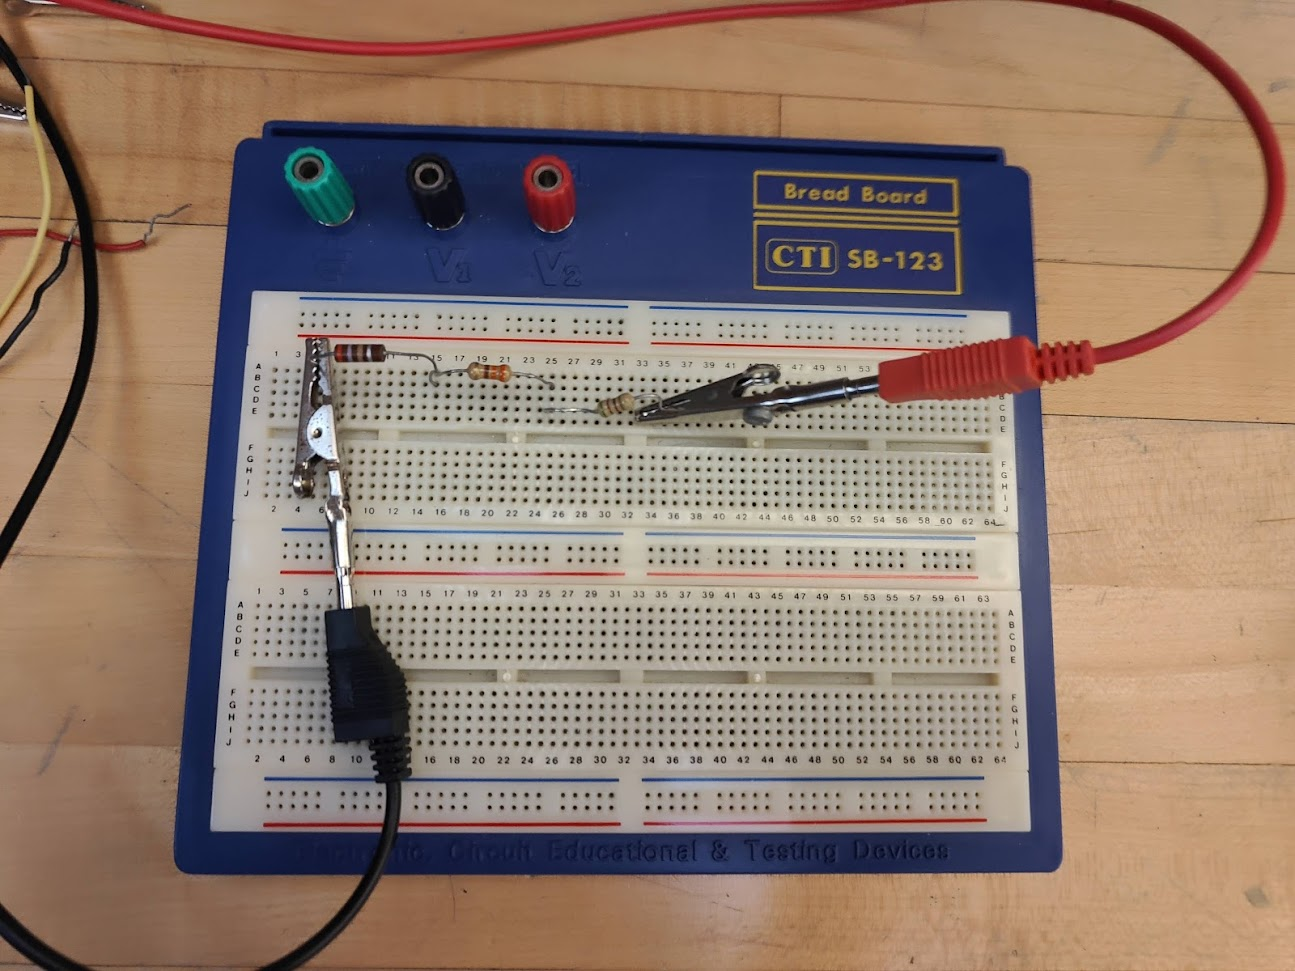
\includegraphics[scale=0.2]{procedure/series} 
        \end{figure}

        \FloatBarrier
        \subsection{Parallel Circuit}
        \FloatBarrier

        \begin{figure}[hbt!]
            \centering
            \caption{Resistors in a parallel configuration}
            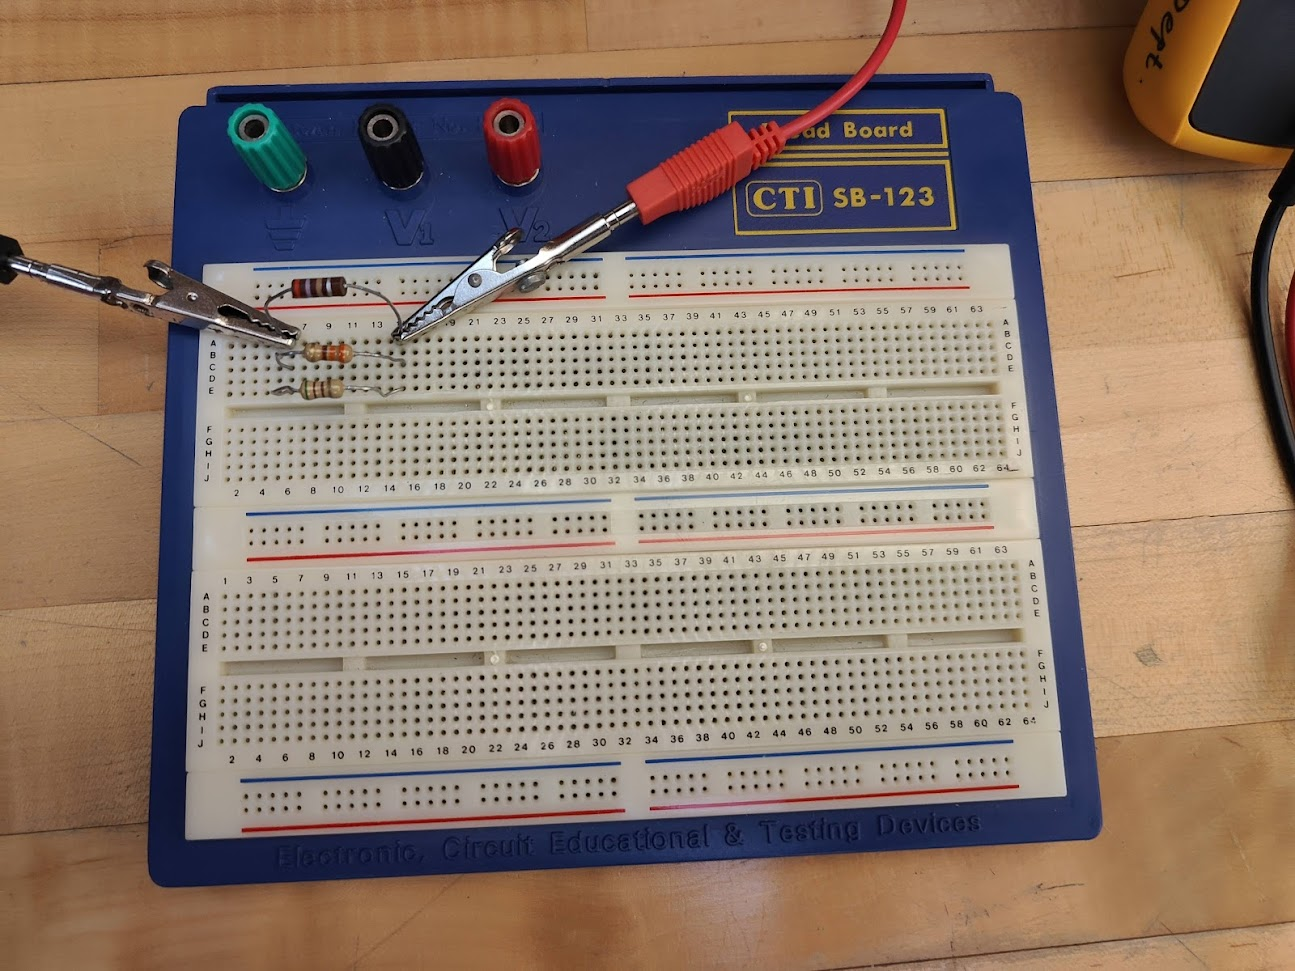
\includegraphics[scale=0.2]{procedure/parallel} 
        \end{figure}



	\section{Data and Graphs}
	\subsection{Value of the Resistor}
		\begin{center}
		\rowcolors{2}{gray!10}{gray!40}
		\begin{tabular}{c|c|c|c|c}
			Resistor & Colors & Expected Resistance (\(\Omega\)) & Actual Resistance (\(\Omega\)) & Percent Error \\
			\hline
			1 &\textcolor{red}{ Blue} \textcolor{blue}{ Grey} Green Silver & 6800k\(\Omega \pm 10\%\) & 7200k\(\Omega\) & 5.88\% \\
			2 & Blue Grey Yellow Silver & 680k\(\Omega \pm 10\%\) & 644k\(\Omega\) & 5.29\% \\
			3 & Red Purple Orange Silver & 27k\(\Omega \pm 10\%\) & 27.35k\(\Omega\) & 1.30\% \\
			4 & Red Red Red Silver & 2200\(\Omega \pm 10\%\) & 2198\(\Omega\) & 0.09\% \\
			5 & Orange Orange Brown Silver & 330\(\Omega \pm 10\%\) & 334.5\(\Omega\) & 1.36\% \\
			6 & Yellow Purple Black Gold & 47\(\Omega \pm 5\%\) & 47.5\(\Omega\) & 1.06\% \\
			
		\end{tabular}
	\end{center}
	\subsection{Series Circuit} 
		\begin{center}
		\rowcolors{2}{gray!10}{gray!40}
		\begin{tabular}{c|c|c}
			Resistor ( \(\Omega\)) & Measured Voltage Drop (V) & Calculated Current (mA) \\
			\hline
			368.2 & 1.2 & 3.26\\
			328.7 & 1.07 & 3.26\\
			521.9 & 1.7 & 3.26
		\end{tabular}
	\end{center}
	\subsection{Parallel Circuit}
		\begin{center}
		\rowcolors{2}{gray!10}{gray!40}
		\begin{tabular}{c|c|c|c}
			Resistor (\(\Omega\)) & Measured Voltage Drop (V) & Calculated Current (mA) & Power Dissipated (W)\\
			\hline
			368.2 & 3.9 & 106 & 0.4134\\
			328.7 & 3.9 & 119 & 0.4641\\
			521.9 & 3.9 & 74.7 & 0.291
		\end{tabular}
	\end{center}
    \section{Calculations \& Results}

        \subsection{Value of the Resistor} 
		In order to find the expected/nominal value of the resistor, Figure 7.1.1 was taken into consideration. Each colored stripe on the resistor corresponded to a digit, magnitude, or tolerance. 
		\begin{center}
		\begin{figure}[h!]
			\caption*{[Fig 7.1.1] 4-band Resistor Color Chart}
			\centering
                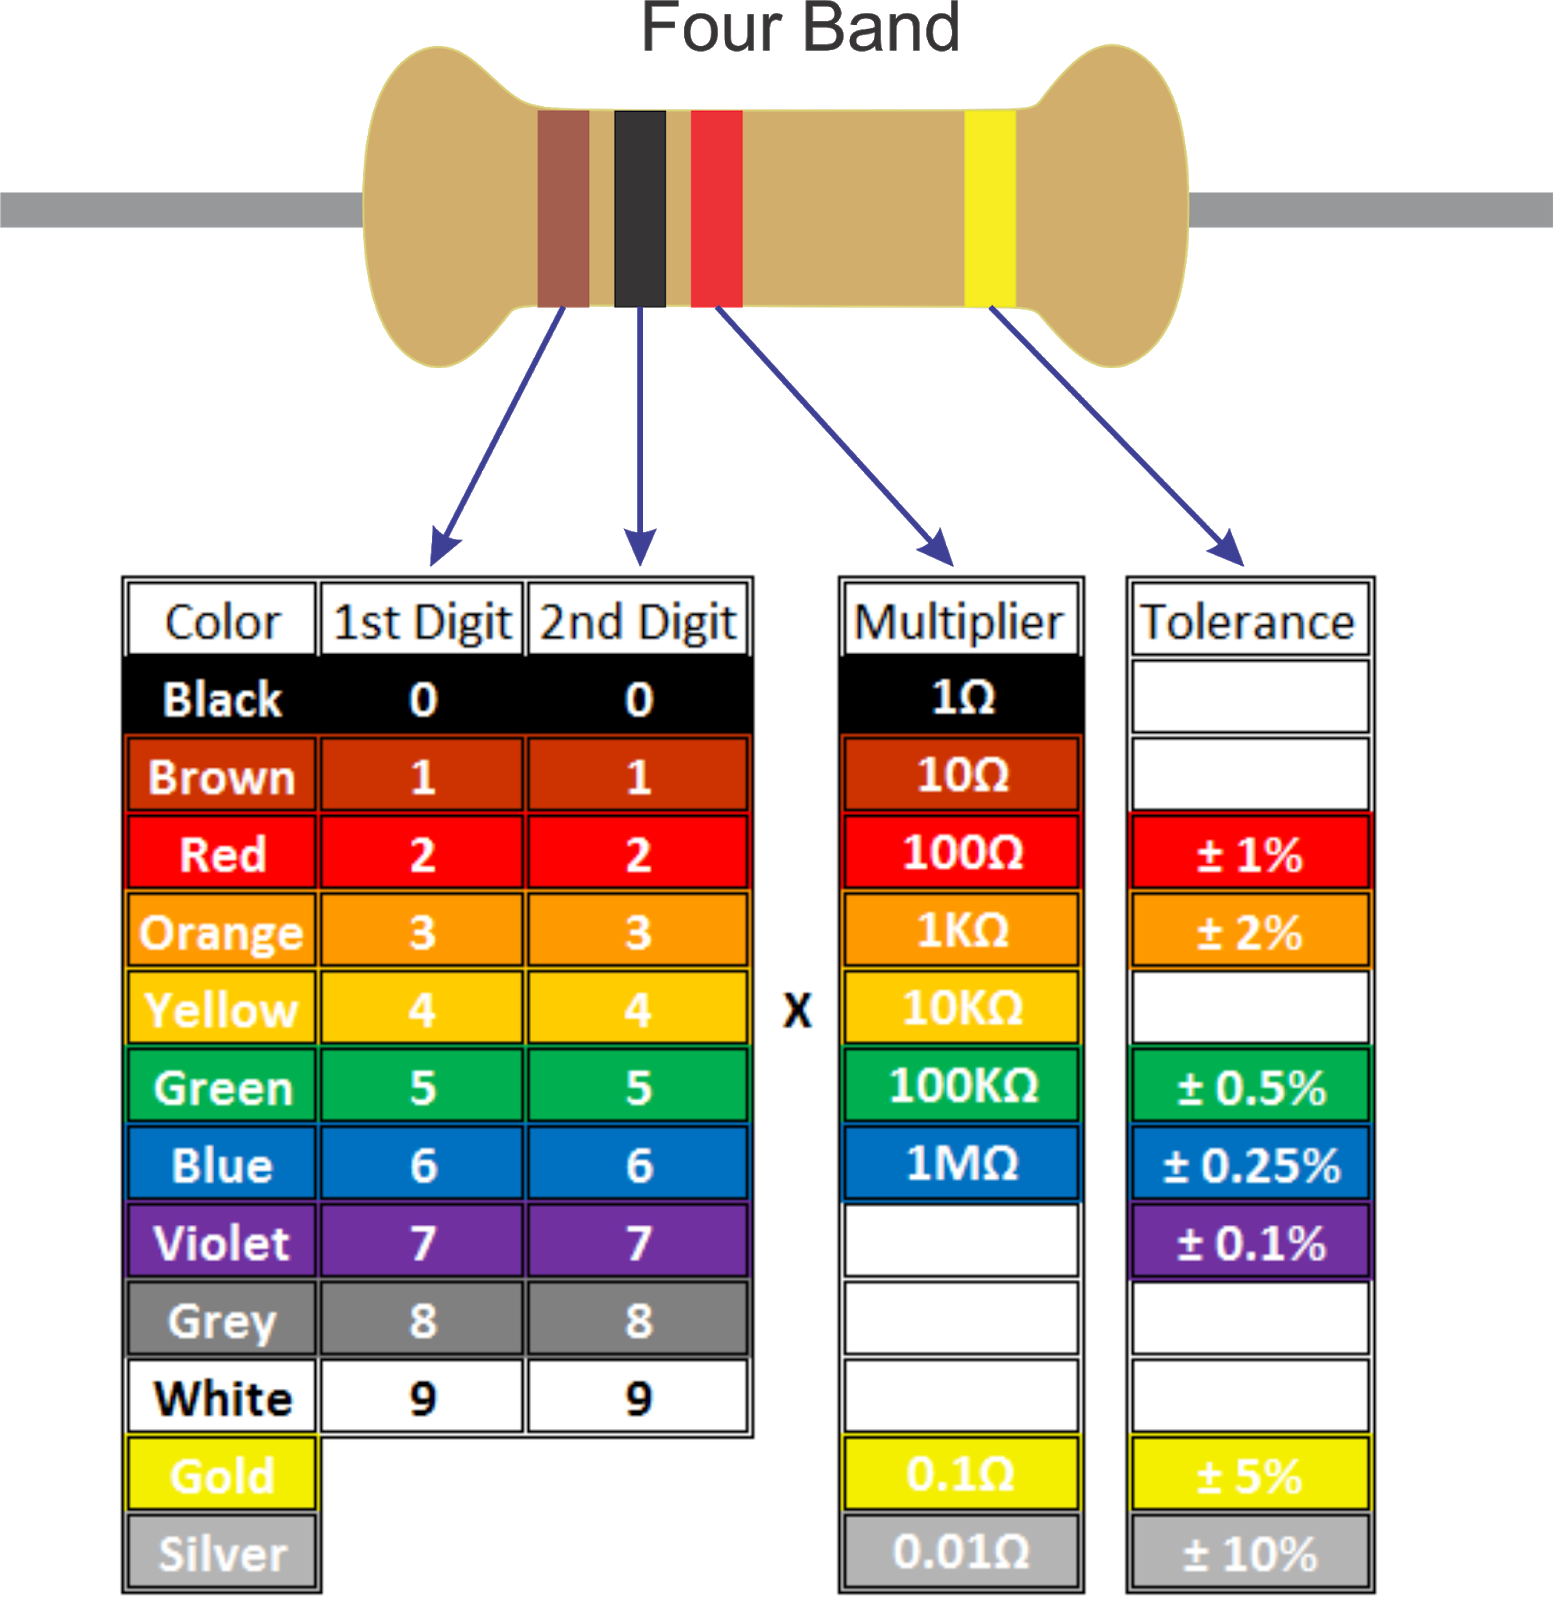
\includegraphics[scale=0.17]{results/band-code.jpg}
	\end{figure}
	\end{center}
The actual resistance was found via the Digital Multimeter on resistor mode, and connecting one lead on each end of the resistor. \\
\vspace{0.5cm}
The percent error was found using the expression
\[\%E = \frac{|\text{Theoretical} - \text{Experimental}|}{\text{Theoretical}} \times 100\]

To check if the resistors are within specification, the tolerance was applied to the nominal value of the resistor. This was done by creating a range of values the resistance could fall into. To find the lower bound, the following equation was used:
\[\text{Lower Bound} = \text{Nominal Resistance} - \left(\frac{\text{Nominal Resistance} \times \text{Tolerance}}{100}\right)\] 
To find the upper bound, the following equation was used:
\[\text{Upper Bound} = \text{Nominal Resistance} + \left(\frac{\text{Nominal Resistance} \times \text{Tolerance}}{100}\right)\] 
Thus, all of the measured resistances fall into the specification range.

        \subsection{Series Circuit} 
	In order to find the current over a specific resistor, the resistance and voltage drop of the resistor is needed. Then, the following equation is applied:
\[ \text{I} = \frac{\text{V}}{\text{R}} \]
To find the equivalent resistance of a circuit in series, the following formula was used:
\[\text{V}_{eq} = \text{R}_{1} + \text{R}_2 + \text{R}_n + ... \]
To find the percent error in the voltage drops compared to the power supply value, the following equation is used:
\[\%E = \frac{|\text{Power Supply Voltage} - \text{Voltage Drop Total}|}{\text{Power Supply Voltage}} \times 100\]

	\subsection{Parallel Circuit}
	In order to find the current over a specific resistor, the resistance and voltage drop of the resistor is needed. Then, the following equation is applied:
\[ \text{I} = \frac{\text{V}}{\text{R}} \]
	To find the power dissipated by each resistor in the circuit, apply the following equation:
	\[ \text{P} = \text{IV}\]
	To find the equivalent resistance of a circuit in parallel, the following formula was used:
	\[\frac{1}{\text{R}_{eq}} = \frac{1}{\text{R}_1} + \frac{1}{\text{R}_2} + \frac{1}{\text{R}_n} + ... \]
	To find the current through the battery, apply the following equation using the battery voltage and the equivalent resistance.
\[ \text{I} = \frac{\text{V}}{\text{R}} \]


\section{Questions}
\subsection*{Part 1 - Measurement of Resistors}
    \begin{enumerate} 
        \item Include here a picture of the set-up of just one measurement of resistance (showing the value in the display of the DMM)
            \begin{figure}[hbt!]
                \centering
                \caption{Resistance measurement setup}
                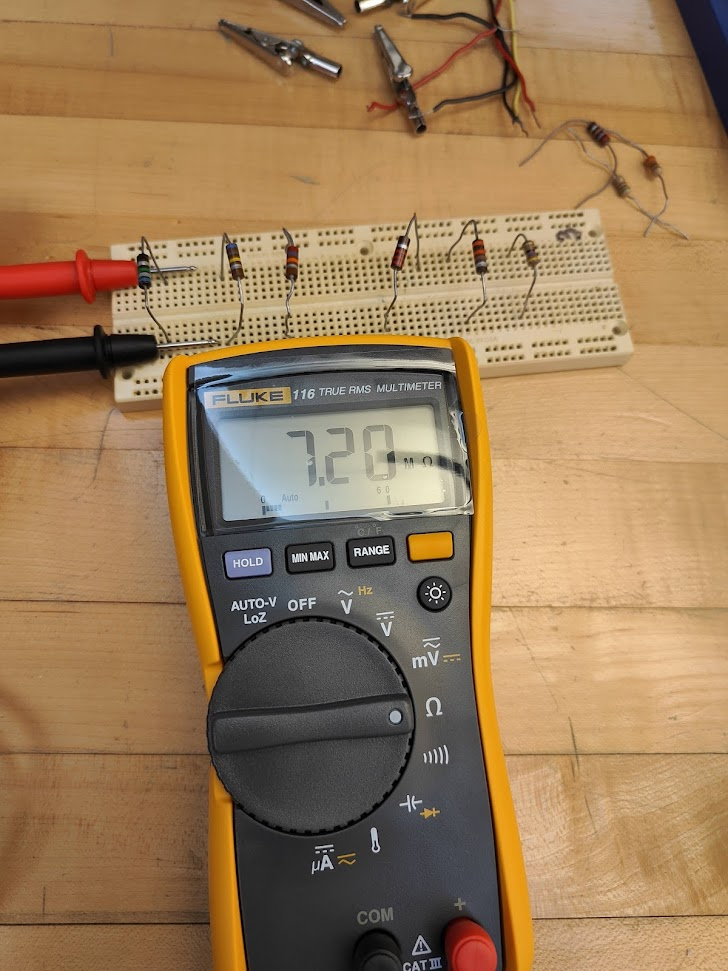
\includegraphics[scale = 0.2]{questions/measurement}
            \end{figure} 
            \\(There is a hand maintaining pressure on the probes for optimal contact just outside of the frame)

        \item Do some research about the meaning of the tolerance (gold or silver colors). Are the resistors within specification? Explain\\
    \end{enumerate}
    \FloatBarrier


\subsection*{Part 2 - Series Circuit} 
    \begin{enumerate} 
        \item Did you get the same value of current across all the resistors? \\ 
            \textbf{Yes sir!}
        \item What is the equivalent resistance of the circuit\\ 
            \textbf{$\mathbf{R_{eq}}$ = 1221.2$\mathbf{\Omega}$ }

        \item Did the voltage drop across the resistors add up to the value of the power supply? What is the percent error?\\ 
            \textbf{Nearly, we had 0.75\% error, off by 0.03 Volts}


    \end{enumerate}

\subsection*{Part 3 - Parallel Circuit} 
    \begin{enumerate} 
        \item Do you obtain the same voltage across each resistor? \\
            \textbf{Yes sir!} 

        \item Calculate the equivalent resistance of the circuit \\
            $$\mathbf{R_{eq} = 1218.8 \Omega}$$
        \item Calculate the current through the battery using the power supply value and the equivalent resistance \\ 
            $$ \mathbf{I=\frac{V}{R} = \frac{4.0V}{1218.8\Omega} =3.28 mA }$$ 
        \item Is the power dissipated through each resistor the same? If no, through what resistor is the power the greatest?\\
            \textbf{No chief, it isn't. R2 has the greatest power dissipation} 
    \end{enumerate}

\subsection*{Part 4 - Series and Parallel Circuit} 
    \FloatBarrier
    \begin{figure}[hbt!]
        \centering
        \caption{Series and parallel circuit diagram}
        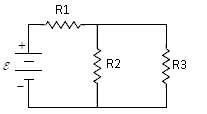
\includegraphics[scale = 1.2]{images/questions/circuit.png}
    \end{figure}
    \FloatBarrier

    \begin{itemize} 
        \item Battery Voltage: $\mathbf{\varepsilon = 3.88V }$ 
        \item Resistor values $$\mathbf{R_1 =368.2\Omega, \text{     } R_2 = 328.7 \Omega , \text{      } R_3 = 521.9 \Omega }$$
        \item What is the equivalent resistance?\\ $$\mathbf{ R_{eq} = 0.575k \Omega}$$

        \item Potential difference across each resistor
        $$\mathbf{V_1 = 2.472V, \text{    } V_2 = 1.406V, \text{    } V_3 = 1.406V}$$
        \item Current flowing through each resistor 
            $$\mathbf{ I_1 = 6.80 mA, \text{   }, I_2 = 4.13 mA, \text{    } I_3 = 2.62 mA }$$
        \item Power dissipated by each resistor 
            $$\mathbf{ P_1 = 16.8mW, P_2 = 5.81 mW, P_3 = 3.68mW }$$
        \item Total current supplied by battery
            $$\mathbf{I_\text{total} = 6.8 mA}$$
    \end{itemize}




	\section{Conclusion}


\end{document}
